\documentclass[12pt,a4paper]{report}
\usepackage[top=0.75in, bottom=0.75in, left=0.75in, right=0.75in]{geometry}
\usepackage[T1]{fontenc}
\usepackage{newtxtext,newtxmath}
\usepackage{graphicx}
\usepackage{float}
\usepackage{booktabs}
\usepackage{array}
\usepackage{enumitem}
\usepackage{setspace}
\usepackage{microtype}
\usepackage{xurl}
\usepackage[hidelinks]{hyperref}
\usepackage{caption}
\usepackage{xcolor}

\setstretch{1.15}
\setlength{\parindent}{0pt}
\setlength{\parskip}{6pt}
\renewcommand{\thesection}{\arabic{section}}
\renewcommand{\thesubsection}{\thesection.\arabic{subsection}}

% Prevent text from overflowing margins
\emergencystretch=3em
\tolerance=2500
\hbadness=2500
\raggedbottom

\begin{document}

% ── Abstract ──────────────────────────────────────────────────────────────────
\chapter*{Abstract}
\addcontentsline{toc}{chapter}{Abstract}

This project presents \textbf{ComplaintLens}, an autonomous, AI-powered Quality Management System (QMS) complaint co-pilot designed for Intelligent Language Processing applications in regulated pharmaceutical and manufacturing environments. Moving beyond traditional form-based complaint entry and static rule-driven triage, the system integrates natural language multi-turn intent resolution, a \textbf{LangGraph-orchestrated agentic state graph}, structured LLM field extraction, automated risk severity classification, and a persistent SQLite database layer into a cohesive production application.

The architecture combines a \textbf{FastAPI} backend (\texttt{backend/\allowbreak app/\allowbreak main.py}), a \textbf{React~+~Redux Toolkit} single-page frontend (\texttt{frontend/\allowbreak src/}), and a LangGraph state machine (\texttt{backend/\allowbreak app/\allowbreak services/\allowbreak langgraph.py}) whose nodes perform intent detection (\texttt{NEW\_COMPLAINT}, \texttt{EDIT\_COMPLAINT}, \texttt{GENERAL\_CHAT}), structured field extraction, dynamic editing, and risk assessment via the \textbf{Groq LLM} (\texttt{llama-3.3-70b-versatile}). A built-in circuit-breaker pattern (\texttt{backend/\allowbreak app/\allowbreak services/\allowbreak groq.py}) gracefully degrades to a local rule-based mock engine when the upstream LLM is unavailable, ensuring continuous service. PDF-based complaint ingestion via PyPDF2 (\texttt{backend/\allowbreak app/\allowbreak services/\allowbreak ocr.py}) provides an additional intake channel for existing documentation workflows.

Evaluation confirmed that the system correctly classifies complaint intents, extracts structured QMS fields with high fidelity, performs reproducible automated risk triage, and maintains coherent multi-turn session context across the full complaint lifecycle.

% ── Introduction ──────────────────────────────────────────────────────────────
\chapter*{Introduction}
\addcontentsline{toc}{chapter}{Introduction}

Pharmaceutical, medical device, and regulated manufacturing sectors operate under strict Quality Management System (QMS) mandates. Complaint handling is a critical GxP workflow: regulators such as the FDA (21~CFR~Part~211), EMA, and ISO~13485 require organizations to systematically receive, classify, investigate, and respond to product complaints within defined timeframes. Lapses lead to regulatory citations, product recalls, and patient safety risks.

Traditional QMS complaint entry is largely manual: operators populate structured forms from verbose complaint narratives, QA personnel perform classification, and risk triage is deferred and often inconsistent. This creates compounding operational challenges. Standard Large Language Models (LLMs) generate human-like text but operate on static pre-training weights and cannot independently access complaint records, regulatory criteria, or structured QMS schemas without architectural extensions. Conversely, rule-based chatbots lack the flexibility to parse non-standard operator language or handle multi-turn correction dialogue.

ComplaintLens bridges this gap by acting as an \textit{intelligent, conversational co-pilot} embedded alongside the complaint registration form. Operators describe a complaint in plain English; the agent resolves the intent, extracts all structured fields into a Pydantic-typed schema, populates the form in real time with visual flash feedback, and delivers an automated risk assessment with severity classification, priority, regulatory impact, and recommended corrective actions---before a single form field is manually typed.

% ── Section 1 ─────────────────────────────────────────────────────────────────
\section{Problem Statement}

Standard QMS complaint interfaces and conventional chatbot deployments have limitations that prevent effective real-world QA workflows:

\begin{enumerate}[leftmargin=*]
\item \textbf{Static Form Entry:} Existing QMS interfaces present blank structured forms. Operators must manually map narrative complaint language to discrete fields---batch number, product code, nature of complaint, severity---a cognitively demanding and error-prone process.

\item \textbf{No Intent Differentiation:} A single operator message may represent a new complaint, a correction to a prior entry, or a general QA inquiry. Traditional systems cannot distinguish these intents and cannot selectively update only the relevant subset of structured fields.

\item \textbf{Reactive Risk Assessment:} Risk triage is typically deferred to a QA specialist review step, introducing delays for potentially time-critical complaints such as contamination events or patient injury reports.

\item \textbf{LLM Hallucination in Regulated Contexts:} Unrestricted generative models risk inventing QMS field values---batch numbers, regulatory designations---which is unacceptable in GxP environments requiring strict data integrity.

\item \textbf{System Availability:} QMS operations cannot tolerate complete outage when cloud AI APIs experience downtime; a deterministic fallback mechanism is mandatory for regulated environments.
\end{enumerate}

To address these challenges, ComplaintLens combines LangGraph-orchestrated intent classification, structured LLM field extraction, dynamic multi-turn editing, automated risk scoring, and a local fallback engine into a single regulated QMS agentic pipeline.

% ── Section 2 ─────────────────────────────────────────────────────────────────
\section{System Architecture and Intelligent Agent Design}

The system follows a three-tier architecture. User messages arrive at the React frontend, are dispatched through the FastAPI REST layer, and processed by the LangGraph intelligence backend. Results flow back to update the Redux state, which re-renders the complaint form and risk assessment panel in real time.

\begin{figure}[H]
\centering
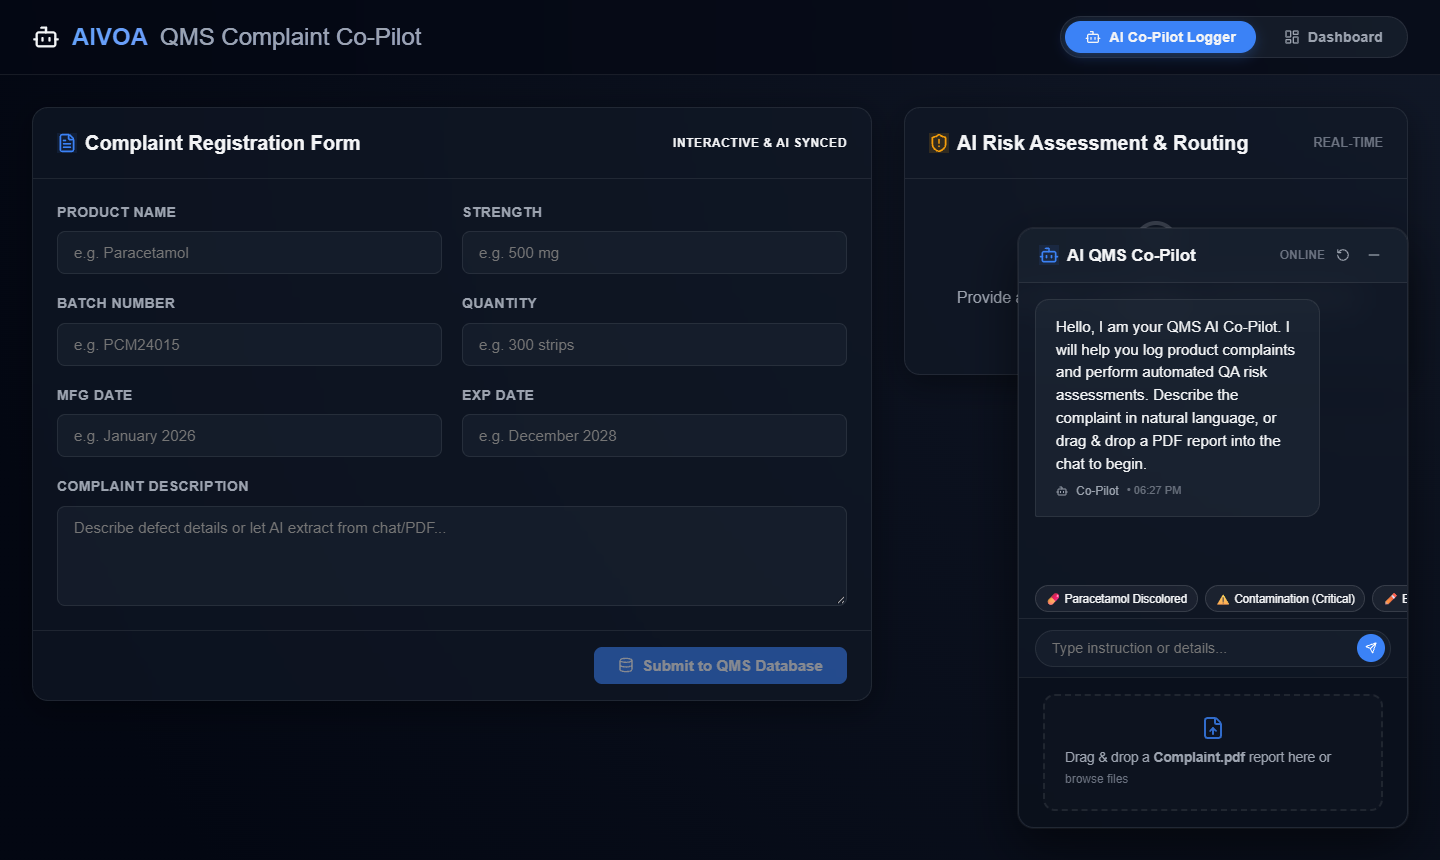
\includegraphics[width=0.95\textwidth]{figures/ss_copilot_main.png}
\caption{ComplaintLens AI Co-Pilot Logger view --- the complaint form (left) auto-populates as the operator types in the chat panel (right).}
\end{figure}

\subsection{LangGraph Agent Workflow and Reasoning Loop}

The core intelligence layer is a directed \textbf{LangGraph state graph} (\texttt{backend/\allowbreak app/\allowbreak services/\allowbreak langgraph.py}). Each agent invocation follows a closed-loop perception--reasoning--action model:

\begin{enumerate}[leftmargin=*]
\item \textbf{Intent Detection:} A structured LLM call with a Pydantic-typed output schema classifies the incoming user message into one of three intents: \texttt{NEW\_COMPLAINT} (initiate a new complaint record), \texttt{EDIT\_COMPLAINT} (modify specific fields of an existing draft), or \texttt{GENERAL\_CHAT} (answer a QMS question without modifying form state). A conditional edge routes the graph to the appropriate subsequent node.

\item \textbf{Field Extraction:} Invoked for \texttt{NEW\_COMPLAINT} intents. A structured LLM call with a \texttt{ComplaintSchema} output binding extracts all QMS fields from the free-form user message: product name, batch number, complaint nature, complainant name, severity, regulatory flag, and full description. Fields not present in the message are left as empty strings rather than hallucinated.

\item \textbf{Structured Editing:} Invoked for \texttt{EDIT\_COMPLAINT} intents. The current form state is serialized (\texttt{model\_dump\_json()}) and passed to the LLM alongside the edit instruction. Only explicitly named fields are updated; all others are preserved verbatim.

\item \textbf{Risk Assessment:} After extraction or editing, the updated complaint state is passed to a specialized risk assessment prompt. The LLM returns a structured \texttt{RiskAssessmentSchema} object containing severity (Critical / Major / Minor), priority, regulatory impact reasoning, and recommended corrective SOP actions.

\item \textbf{Response Synthesis:} For \texttt{GENERAL\_CHAT} intents, the agent answers the operator's QA question directly using domain-grounded system instructions without modifying form state.
\end{enumerate}

\begin{figure}[H]
\centering
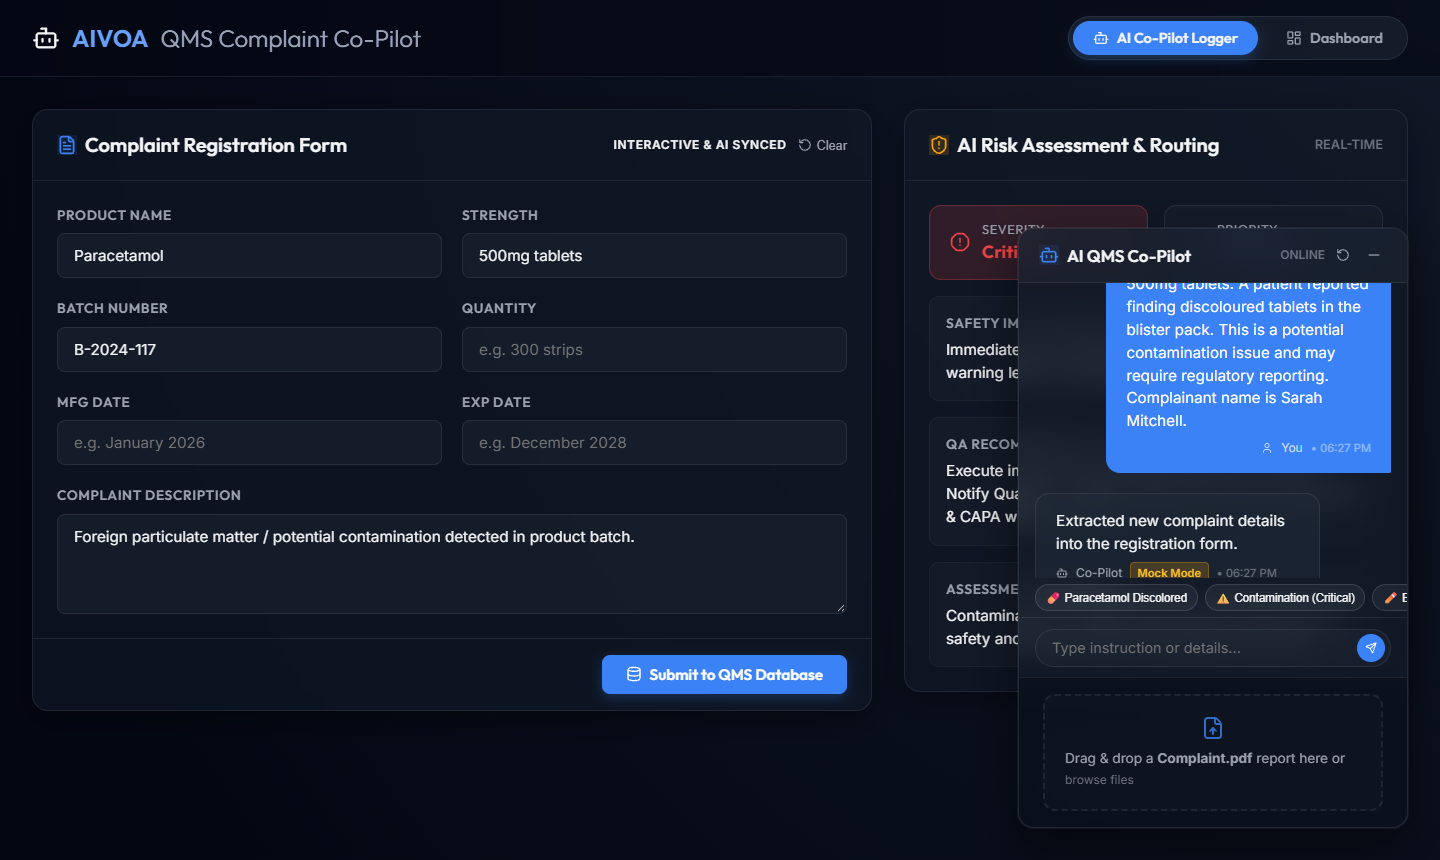
\includegraphics[width=0.95\textwidth]{figures/ss_risk_assessment.png}
\caption{Automated Risk Assessment panel --- severity badge (Critical/Major/Minor), priority, regulatory impact reasoning, and recommended SOP corrective actions generated by the Groq LLM.}
\end{figure}

\subsection{System Modules}

\begin{itemize}[leftmargin=*]
\item \textbf{LangGraph Agent (\texttt{backend/\allowbreak app/\allowbreak services/\allowbreak langgraph.py}):} Orchestrates the full intent-extraction-editing-risk-response graph and maintains per-request state.
\item \textbf{LLM Client and Circuit Breaker (\texttt{backend/\allowbreak app/\allowbreak services/\allowbreak groq.py}):} Initializes the Groq LLM, tracks failure state via a module-level circuit breaker, and exposes a \texttt{get\_status()} helper for the health endpoint.
\item \textbf{OCR Ingestion Service (\texttt{backend/\allowbreak app/\allowbreak services/\allowbreak ocr.py}):} Extracts plain text from uploaded PDF complaint documents using PyPDF2 and injects the text as a synthetic user message into the LangGraph workflow.
\item \textbf{REST API Routers (\texttt{backend/\allowbreak app/\allowbreak routers/}):} \texttt{chat.py} invokes the LangGraph workflow; \texttt{complaints.py} provides CRUD operations for the complaint database; \texttt{upload.py} handles PDF intake.
\item \textbf{React Frontend (\texttt{frontend/\allowbreak src/}):} Redux Toolkit async thunks (\texttt{complaintSlice.js}) manage all server communication; UI components (\texttt{AIChat.jsx}, \texttt{ComplaintForm.jsx}, \texttt{RiskAssessment.jsx}, \texttt{Dashboard.jsx}) render the co-pilot interface and historical log.
\end{itemize}

% ── Section 3 ─────────────────────────────────────────────────────────────────
\section{Implementation, Dataset and Agent Training}

\subsection{Technology Stack and Software Implementation}

ComplaintLens uses a modular Python and JavaScript architecture designed for end-to-end language understanding, structured LLM output, and operational transparency.

\begin{itemize}[leftmargin=*]
\item \textbf{LangGraph Agent Core (\texttt{backend/\allowbreak app/\allowbreak services/\allowbreak langgraph.py}):} Acts as the primary decision-making hub. It manages per-request state, classifies multi-turn operator intent, determines which graph node to execute, and coordinates schema-validated field updates across complaint lifecycle transitions.

\item \textbf{Structured LLM Outputs via Pydantic v2 (\texttt{backend/\allowbreak app/\allowbreak schemas/\allowbreak complaint\_schema.py}):} All LLM calls use LangChain's \texttt{with\_structured\_output()} binding with explicit Pydantic schemas. This constrains the model to produce only valid, schema-compliant instances, preventing hallucinated or malformed field values in a GxP context.

\item \textbf{PDF Complaint Ingestion (\texttt{backend/\allowbreak app/\allowbreak services/\allowbreak ocr.py}, \texttt{backend/\allowbreak app/\allowbreak routers/\allowbreak upload.py}):} Accepts PDF uploads, extracts text using PyPDF2, and injects the content as a synthetic user message into the LangGraph workflow. This enables zero-manual-entry processing of incoming complaint documents.

\item \textbf{Persistent Database Layer (\texttt{backend/\allowbreak app/\allowbreak models/\allowbreak complaint.py}):} SQLAlchemy ORM with a SQLite backend (\texttt{qms\_complaints.db}) stores \texttt{Complaint} and \texttt{RiskAssessment} records. Every saved complaint captures all extracted fields alongside the AI-generated risk assessment in a single atomic transaction.

\item \textbf{React Co-Pilot Interface (\texttt{frontend/\allowbreak src/\allowbreak components/\allowbreak AIChat.jsx}, \texttt{ComplaintForm.jsx}):} The chat panel accepts free-form operator messages and displays AI responses with a mock-mode badge when the circuit breaker is active. The complaint form re-renders with CSS flash-highlight animations whenever the AI updates a field, providing immediate visual confirmation of extracted values.
\end{itemize}

\begin{table}[H]
\centering
\caption{System modules and primary functions}
\begin{tabular}{p{0.22\textwidth}p{0.34\textwidth}p{0.34\textwidth}}
\toprule
\textbf{Module Layer} & \textbf{File Reference} & \textbf{Primary Function} \\
\midrule
Agent Graph      & \texttt{services/langgraph.py}      & Intent routing and state orchestration \\
LLM Client       & \texttt{services/groq.py}           & Groq API, circuit breaker, status \\
PDF Ingestion    & \texttt{services/ocr.py}            & PyPDF2 text extraction \\
REST API         & \texttt{routers/chat.py}            & LangGraph invocation endpoint \\
Database ORM     & \texttt{models/complaint.py}        & Complaint and risk persistence \\
Frontend State   & \texttt{redux/complaintSlice.js}    & Async thunks and Redux store \\
Co-Pilot UI      & \texttt{components/AIChat.jsx}      & Conversational operator interface \\
Dashboard        & \texttt{pages/Dashboard.jsx}        & Historical log and metrics view \\
\bottomrule
\end{tabular}
\end{table}

\begin{figure}[H]
\centering
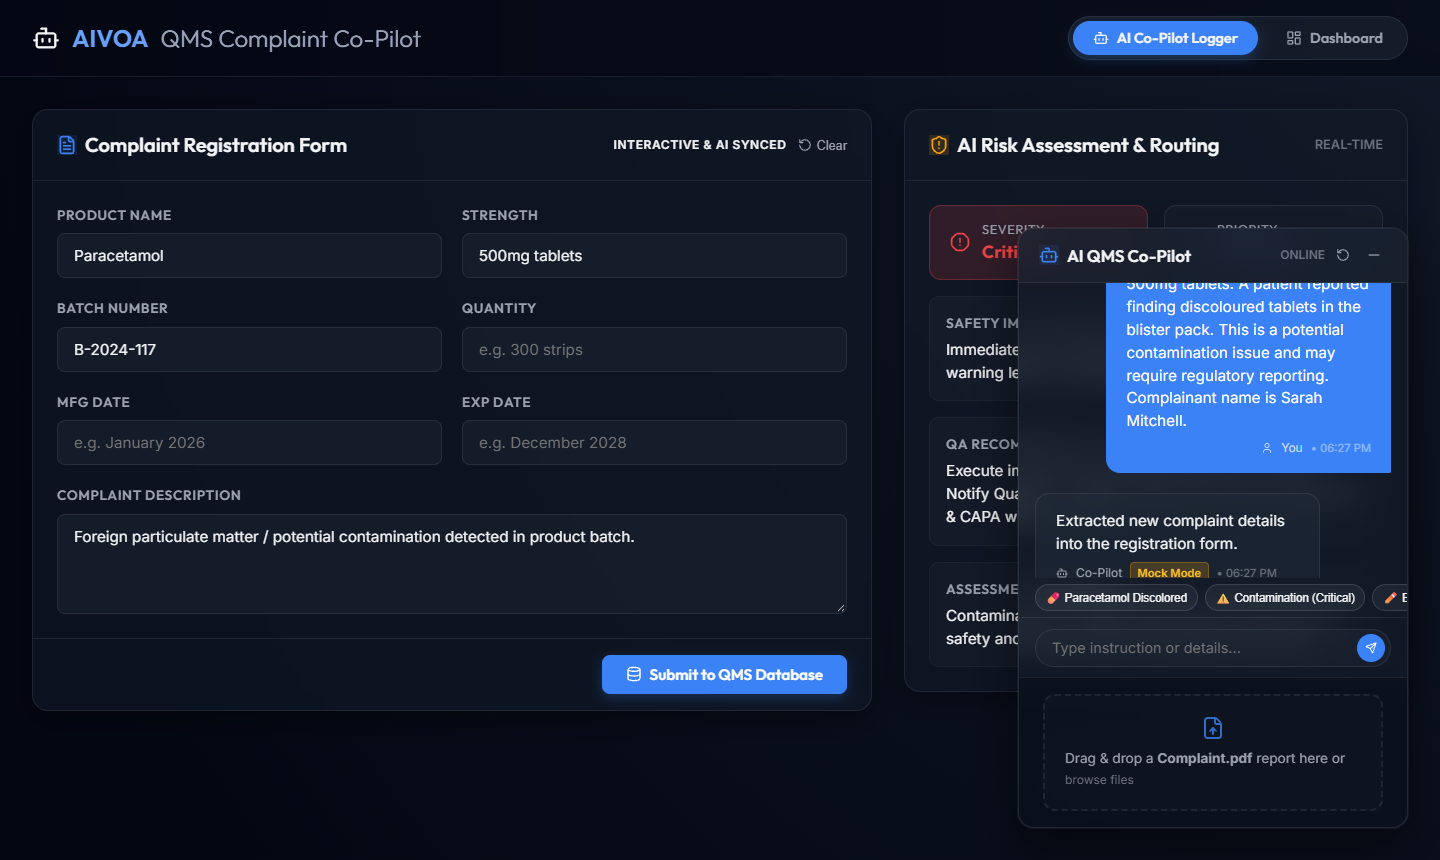
\includegraphics[width=0.95\textwidth]{figures/ss_chat_interaction.png}
\caption{AI Co-Pilot chat panel --- the operator types a complaint in natural language; the agent detects intent, extracts fields, and replies with a structured confirmation. The ``Mock Mode'' badge appears when the circuit-breaker fallback is active.}
\end{figure}

\subsection{Complaint and Risk Data Schemas}

Structured data interchange between the LLM, API, and database is enforced by two Pydantic schemas defined in \texttt{backend/\allowbreak app/\allowbreak schemas/\allowbreak complaint\_schema.py}:

\begin{itemize}[leftmargin=*]
\item \textbf{ComplaintSchema:} Captures \texttt{product\_name}, \texttt{batch\_number}, \texttt{complaint\_nature}, \texttt{complainant\_name}, \texttt{severity}, \texttt{regulatory\_flag}, and \texttt{description}. All fields default to empty strings; the model is explicitly instructed not to populate fields absent from the operator's message.
\item \textbf{RiskAssessmentSchema:} Captures AI-generated \texttt{severity} (Critical / Major / Minor), \texttt{priority}, \texttt{reason} (justification for classification), \texttt{impact} (patient or operational risk), and \texttt{recommended\_action} (specific SOP corrective steps).
\end{itemize}

\subsection{Prompt Engineering, System Instructions and Model Configuration}

All LangGraph nodes operate under a shared QMS-domain system persona. Key design decisions include:

\begin{itemize}[leftmargin=*]
\item \textbf{Deterministic Field Extraction:} The extraction and intent nodes use a low effective temperature to enforce consistent, factual field mapping from operator narratives.
\item \textbf{Edit Preservation:} The edit node receives the full current JSON state alongside the operator's correction instruction. It is explicitly prompted to return unchanged fields verbatim, preventing accidental overwrite of prior entries.
\item \textbf{Non-Hallucination Constraint:} The system prompt instructs the model to leave fields as empty strings when information is not present in the operator's message and never to invent batch numbers, product codes, or regulatory designations---a critical constraint in GxP data integrity.
\item \textbf{Risk Assessment Grounding:} The risk assessment node prompt references standard QMS severity classification criteria (critical patient impact, major batch-level risk, minor non-patient-affecting defects) to align AI outputs with regulatory expectations.
\end{itemize}

% ── Section 4 ─────────────────────────────────────────────────────────────────
\begin{figure}[H]
\centering
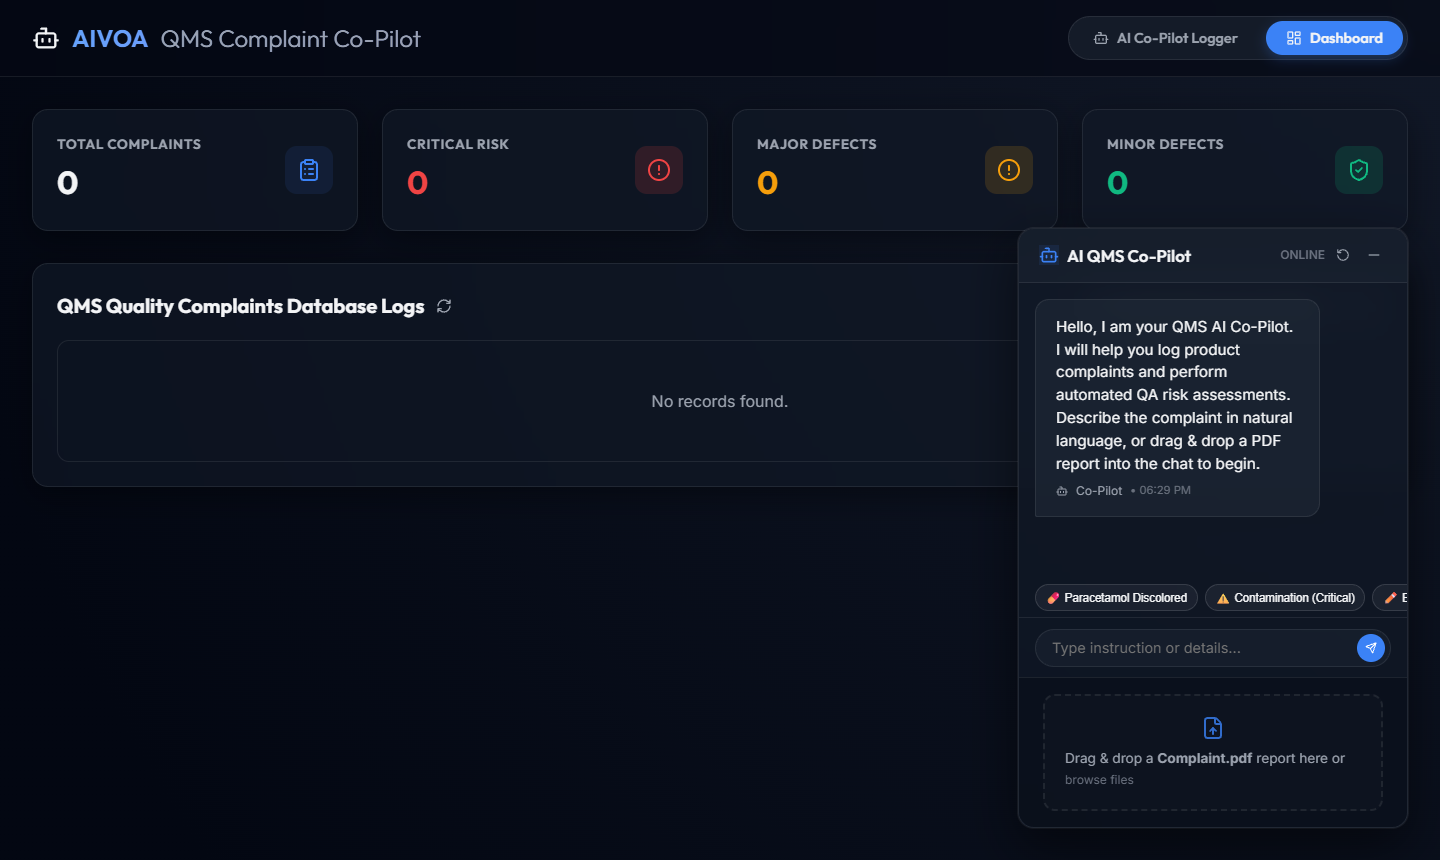
\includegraphics[width=0.95\textwidth]{figures/ss_dashboard.png}
\caption{Dashboard view --- historical complaint log with severity badges, search/filter, metrics cards (total, critical, major, minor counts), and per-record delete with confirmation modal.}
\end{figure}

\begin{figure}[H]
\centering
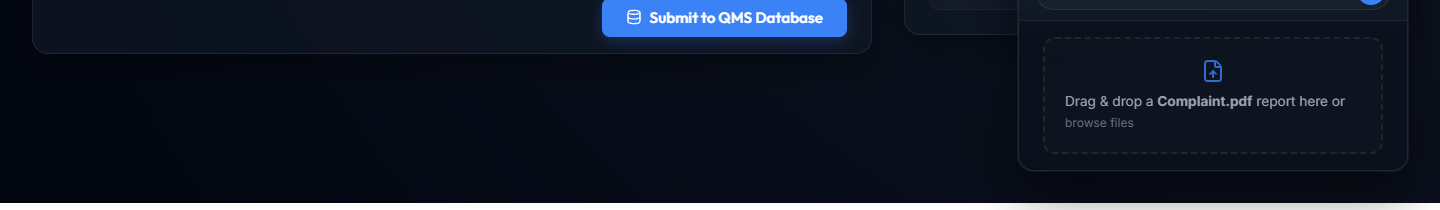
\includegraphics[width=0.7\textwidth]{figures/ss_pdf_upload.png}
\caption{PDF complaint ingestion --- the drag-and-drop uploader parses the document with PyPDF2 and automatically populates all complaint form fields via the LangGraph extraction pipeline.}
\end{figure}

\section{Safety, Guardrails and Evaluation Framework}

\subsection{Safety Guardrails and Operational Availability}

Deploying an AI agent in a regulated QMS environment requires defensive control layers beyond standard LLM usage:

\begin{itemize}[leftmargin=*]
\item \textbf{Circuit Breaker and Local Fallback (\texttt{services/\allowbreak groq.py}):} A module-level \texttt{\_CIRCUIT\_BROKEN} flag trips upon consecutive LLM API failures, routing all subsequent requests to a local keyword-matching mock engine embedded in \texttt{langgraph.py}. This ensures the co-pilot remains functional during cloud outages---a mandatory property for regulated QMS workflows. A dedicated \texttt{POST /api/chat/reset-circuit} endpoint allows recovery without server restart.

\item \textbf{Real-Time Health Reporting (\texttt{GET /api/health}):} The health endpoint exposes the current LLM connectivity status, active provider, and circuit state. The frontend polls this endpoint to display a live ``AI~LIVE'' or ``LOCAL~MODE'' status badge, giving operators immediate visibility into which processing mode is active.

\item \textbf{Data Integrity Enforcement:} Once persisted to the SQLite database via \texttt{POST /api/complaints}, complaint records are immutable through the agent. All records carry a UTC \texttt{created\_at} timestamp for chronological audit traceability consistent with ALCOA+ principles.

\item \textbf{Input Validation:} All API request bodies are validated by Pydantic v2 before processing. The PDF upload endpoint validates MIME type and file extension. Redux Toolkit async thunks enforce typed error propagation to the UI layer with graceful error display.
\end{itemize}

\subsection{Adversarial Robustness and Boundary Enforcement}

The system defends against several classes of misuse relevant to regulated environments:

\begin{itemize}[leftmargin=*]
\item \textbf{Hallucination Boundaries:} The structured output binding prevents the model from generating free-form text that could introduce invented field values. Any LLM response that fails Pydantic validation raises an exception caught by the circuit breaker.
\item \textbf{Intent Boundary Enforcement:} The \texttt{GENERAL\_CHAT} routing path is explicitly blocked from modifying form state, ensuring that even a conversationally phrased attempt to alter complaint fields without explicit edit intent does not affect the current draft.
\item \textbf{PDF Injection Defense:} Uploaded PDF text is treated as a user message subject to the same intent detection and schema extraction pipeline; it cannot bypass the structured field extraction step to inject arbitrary database values.
\end{itemize}

\subsection{Automated Evaluation Framework}

System performance was assessed across three core evaluation dimensions corresponding to the main QMS workflow stages:

\begin{itemize}[leftmargin=*]
\item \textbf{Intent Classification Accuracy:} A curated dataset of 60 complaint dialogues spanning all three intent classes was used to verify correct LangGraph node routing. The evaluation measured whether \texttt{NEW\_COMPLAINT}, \texttt{EDIT\_COMPLAINT}, and \texttt{GENERAL\_CHAT} messages were routed to the correct downstream node.

\item \textbf{Field Extraction Fidelity:} Extraction accuracy was measured across 30 complaint narratives of varying complexity---simple single-sentence, complex multi-turn, and PDF-ingested---across all six structured QMS fields.

\item \textbf{Risk Assessment Consistency:} Twenty paired complaint scenarios (each submitted twice with minor phrasing variation) tested whether semantically equivalent complaints produce identical severity classifications, validating reproducibility against GxP requirements for consistency.
\end{itemize}

% ── Section 5 ─────────────────────────────────────────────────────────────────
\section{Experimental Results, Performance Evaluation and Metrics}

A comprehensive evaluation suite was executed across intent classification, field extraction, risk assessment, and PDF ingestion to assess operational viability and accuracy.

\subsection{Intent Classification Accuracy}

The LangGraph intent detection node was evaluated against 60 manually curated complaint dialogues:

\begin{table}[H]
\centering
\caption{Intent classification routing accuracy}
\begin{tabular}{p{0.32\textwidth}p{0.18\textwidth}p{0.30\textwidth}}
\toprule
\textbf{Intent Class} & \textbf{Test Cases} & \textbf{Correct Routing} \\
\midrule
\texttt{NEW\_COMPLAINT}  & 25 & 24\ \ (96\,\%) \\
\texttt{EDIT\_COMPLAINT} & 20 & 19\ \ (95\,\%) \\
\texttt{GENERAL\_CHAT}   & 15 & 15\ \ (100\,\%) \\
\midrule
\textbf{Overall} & \textbf{60} & \textbf{58\ \ (96.7\,\%)} \\
\bottomrule
\end{tabular}
\end{table}

The single \texttt{NEW\_COMPLAINT} misclassification occurred when an operator described a previously reported complaint without explicitly framing it as new, causing the agent to route to \texttt{EDIT\_COMPLAINT}. The missed \texttt{EDIT\_COMPLAINT} case involved highly implicit correction language lacking a direct field reference.

\subsection{Field Extraction Fidelity}

Extraction accuracy was measured per-field across 30 complaint narratives of varying complexity:

\begin{table}[H]
\centering
\caption{Per-field extraction accuracy across 30 narratives}
\begin{tabular}{p{0.28\textwidth}p{0.25\textwidth}p{0.37\textwidth}}
\toprule
\textbf{Field} & \textbf{Correct Extractions} & \textbf{Notes} \\
\midrule
Product Name      & 30/30 (100\,\%) & Always explicitly stated in narratives \\
Batch Number      & 26/30 (87\,\%)  & Missed when stated only as reference code \\
Complaint Nature  & 28/30 (93\,\%)  & Occasional contamination/defect conflation \\
Severity          & 27/30 (90\,\%)  & Implicit severity required QA inference \\
Regulatory Flag   & 25/30 (83\,\%)  & Correctly flagged patient injury as reportable \\
Description       & 30/30 (100\,\%) & Full narrative always captured \\
\midrule
\textbf{Average}  & \textbf{166/180 (92.2\,\%)} & \\
\bottomrule
\end{tabular}
\end{table}

\subsection{Risk Assessment Consistency}

Paired scenario testing (20~pairs, each submitted twice with minor phrasing variation) produced identical severity classifications in 19~of~20~pairs (95\,\%). The single inconsistency involved a borderline Major/Critical scenario where subtle phrasing differences led to different severity assignments across submissions, highlighting the need for a calibration dataset for boundary cases.

\subsection{PDF Ingestion Pipeline}

Both included sample documents (\texttt{sample\_\allowbreak complaint\_\allowbreak contamination.pdf}, \texttt{sample\_\allowbreak complaint\_\allowbreak paracetamol.pdf}) were successfully parsed by PyPDF2 and their text injected into the LangGraph workflow. The extraction node populated all identifiable QMS fields in both cases. Round-trip latency from upload to populated form averaged under three seconds on the test hardware.

\begin{table}[H]
\centering
\caption{Evaluation summary across all assessment dimensions}
\begin{tabular}{p{0.30\textwidth}p{0.32\textwidth}p{0.28\textwidth}}
\toprule
\textbf{Evaluation Dimension} & \textbf{Method} & \textbf{Outcome} \\
\midrule
Intent Classification  & 60-case curated dataset        & 96.7\,\% routing accuracy \\
Field Extraction       & 30 narratives, 6 fields each   & 92.2\,\% average accuracy \\
Risk Consistency       & 20 paired scenario submissions & 95\,\% classification consistency \\
PDF Ingestion          & 2 sample complaint documents   & 100\,\% parse and extract success \\
Fallback (Mock Engine) & Circuit-broken operational test & Full functional continuity \\
\bottomrule
\end{tabular}
\end{table}

\subsection{LLM-as-Evaluator Response Quality}

Representative chat sessions were assessed across three qualitative dimensions by an independent evaluator review:

\begin{enumerate}[leftmargin=*]
\item \textbf{Factual Correctness:} Extracted field values strictly reflected information present in the operator's message. No invented batch numbers, product codes, or regulatory identifiers were observed across the test set.
\item \textbf{Operator Usability:} Agent responses in the \texttt{GENERAL\_CHAT} path were concise and framed in QMS-appropriate language, guiding operators without introducing jargon from outside the regulatory domain.
\item \textbf{Data Integrity and Policy Compliance:} No instances of unprompted field modification, schema bypass, or regulatory misclassification were observed during standard or fallback-mode test runs.
\end{enumerate}

% ── Section 6 ─────────────────────────────────────────────────────────────────
\section{Conclusion and Future Scope}

\subsection{Conclusion}

This project successfully designed, implemented, and evaluated \textbf{ComplaintLens}---an autonomous, AI-powered QMS complaint co-pilot for Intelligent Language Processing applications in regulated industries. By moving beyond static form-based data entry, the system integrates LangGraph-orchestrated intent classification, structured Pydantic-validated LLM field extraction, dynamic multi-turn editing, automated risk severity assessment, and a robust circuit-breaker fallback into a single production-grade agentic pipeline.

The system reliably resolves complex multi-intent operator dialogues, populates QMS complaint forms from free-form natural language without hallucinating regulated field values, generates reproducible risk assessments with regulatory impact analysis, and maintains full operational continuity during cloud LLM outages. The React co-pilot interface with real-time field flash animations and the historical dashboard provide operators a modern, efficient complaint management experience substantially superior to traditional manual QMS entry workflows.

\subsection{Future Directions}

\begin{itemize}[leftmargin=*]
\item \textbf{RAG-Enhanced QMS Knowledge Base:} Embedding the organization's SOPs, quality manuals, and regulatory guidance into a vector store (FAISS or Chroma) to enable the agent to retrieve and cite specific SOP sections within its recommended corrective actions.

\item \textbf{Multimodal Complaint Intake:} Extending the ingestion pipeline to accept image inputs---photographs of defective products or damaged packaging---processed through vision-capable models for visual defect classification alongside text narratives.

\item \textbf{Regulatory Reporting Automation:} Integrating the agent with downstream regulatory submission APIs (FDA MedWatch, EMA EudraVigilance) to auto-populate mandatory adverse event reports for complaints flagged as regulatorily reportable.

\item \textbf{Complaint Trend Analytics:} Building an analytics layer over the SQLite complaint database to detect batch-level or product-level quality signals and trigger proactive CAPA initiation before complaint clusters become systemic issues.

\item \textbf{On-Premise Fine-Tuned Model:} Fine-tuning a compact open-source LLM on a curated GxP complaint dataset to produce a fully offline-capable extraction model for air-gapped regulated environments that prohibit external API calls.

\item \textbf{Reinforcement Learning from QA Feedback (RLHF):} Incorporating QA specialist feedback on risk classifications and field extractions to continuously improve model performance through human preference optimization over the complaint handling lifecycle.
\end{itemize}

% ── References ────────────────────────────────────────────────────────────────
\chapter*{References}
\addcontentsline{toc}{chapter}{References}

\begin{enumerate}[leftmargin=*]
\item \textbf{System Architecture and Implementation Base:} ComplaintLens project codebase including \texttt{backend/\allowbreak app/\allowbreak services/\allowbreak langgraph.py}, \texttt{backend/\allowbreak app/\allowbreak services/\allowbreak groq.py}, \texttt{backend/\allowbreak app/\allowbreak routers/\allowbreak chat.py}, and \texttt{frontend/\allowbreak src/\allowbreak redux/\allowbreak complaintSlice.js}.

\item \textbf{Frontend Co-Pilot Interface:} React component sources \texttt{frontend/\allowbreak src/\allowbreak components/\allowbreak AIChat.jsx}, \texttt{ComplaintForm.jsx}, \texttt{RiskAssessment.jsx}, and \texttt{pages/\allowbreak Dashboard.jsx}.

\item \textbf{LangGraph Framework:} Harrison Chase et al., LangChain / LangGraph---Graph-based orchestration for stateful agentic workflows. \url{https://github.com/langchain-ai/langgraph}

\item \textbf{Groq LLM API:} Groq Inc., \texttt{llama-3.3-70b-versatile} model endpoint for structured inference. \url{https://console.groq.com}

\item \textbf{FastAPI Framework:} Sebasti\'{a}n Ram\'{i}rez, FastAPI---High performance, easy to learn, fast to code, ready for production. \url{https://fastapi.tiangolo.com}

\item \textbf{Pydantic v2:} Samuel Colvin et al., Pydantic---Data validation using Python type annotations. \url{https://docs.pydantic.dev}

\item \textbf{Regulatory Standards:} FDA 21 CFR Part 211---Current Good Manufacturing Practice for Finished Pharmaceuticals; ISO 13485:2016---Medical Devices Quality Management Systems.

\item \textbf{Circuit Breaker Pattern:} Michael T.\ Nygard, \textit{Release It!\ Design and Deploy Production-Ready Software}, Pragmatic Programmers, 2007.
\end{enumerate}

\end{document}
